


\documentclass[spanish, a4paper, 12pt]{article} 	%idioma, tamaño, tamaño letra, tipo de documento (articulo, libro, report)
\usepackage[english, activeacute]{babel}		%babel para tildes: á = \´{a}	
\usepackage[utf8]{inputenc}
\usepackage{geometry}
\usepackage{multicol}
\usepackage{amsmath}
\usepackage{amssymb}
%\usepackage{amsttthm}
\usepackage{graphics}
\usepackage{graphicx}
\usepackage{hyperref}
\usepackage{wrapfig} 

\usepackage{fancyhdr}
\geometry{a4paper, textwidth=16cm, textheight=20cm}
\pagestyle{fancy}
%\usepackage{nicefrac}
%\setlenght{\parskip}{1}
\lhead{Inteligencia Artificial}
\cfoot{\thepage}
\renewcommand{\headrulewidth}{0.4pt}
\renewcommand{\footrulewidth}{0.4pt}

\begin{document}
\title{\textbf{Inteligencia Artificial}}
\maketitle

\begin{center}
{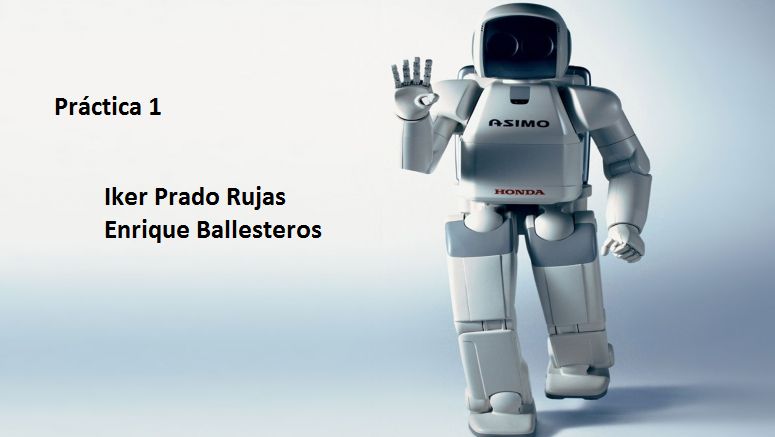
\includegraphics[width=\textwidth]{robotHonda.png}}
\end{center}

\newpage
\textbf{{¿Qué es la inteligencia artificial?}}


\begin{section}{Bots inteligentes de ayuda}

	\begin{itemize}
	
	%\begin{section}{Irene}
	\item{Irene}
	
	Básicamente solo es capaz de analizar frases sencillas, con una estructura concreta y siempre relacionadas con su campo.
	 Aunque también te saluda y se aprende tu nombre. Es más práctico buscar tú los billetes o usar un buscador porque 
	 cuando le preguntas sobre el billete más barato o el tren más rápido no sabe ayudarte.
	 Tiene una guía de uso pero es demasiado optimista creemos: \url{www.renfe.com/empresa/ayudav.html}
	 
	%\end{section}
	%\begin{section}{Anna}
	\item{Anna}
	
	Resumo su funcionamiento en esta conversación:
	
	-Anna ha dicho: Hola, soy Anna, asistente virtual de IKEA. Estoy aquí para ayudarte a mejorar tu experiencia con la página 		web de IKEA, productos y servicios. Hazme una pregunta, y yo te proporcionaré la respuesta más apropiada. 
¿Cómo funciono? Siempre trata de escribir frases cortas, y sólo una a la vez. Cuanto más larga sea tu pregunta, la posibilidad de darte una respuesta incorrecta incrementará. A veces abro una página web con información referente a tu pregunta y mis respuestas pueden tener enlaces en las que puedes pulsar, si lo haces llegarás a respuestas adicionales, con información relacionada. Me encanta aprender, así que si tu pregunta no está en mi base de datos, voy a solicitar que se la agregue a mi conocimiento, tan pronto como sea posible. Tus comentarios serán muy apreciados! Ahora vamos a tener una charla, ¿de acuerdo?

	+Has dicho: De acuerdo.
	
	-Anna ha dicho: Lo siento, no he entendido bien lo que has dicho.
	
	Con esto basta para darse cuenta que está lejos de poder ser denominado inteligencia artificial.
	%\end{section}
	%\begin{section}
	
	\newpage
		\item{Alice}
		
		Realmente de las cuatro es la única que puede considerarse inteligencia artificial.
		Solo pondremos conversaciones con ella, pues son las más interesantes.
		
		\begin{itemize}
			\item{Diferencias entre quién eres y qué eres:}
			
			-judge: how are you? 
			
			+ALICE: My logic and cognitive functions are normal. 
			
			-judge: who are you? 
			
			+ALICE: ALICE. 
			
			-judge: What are you? 
			
			+ALICE: I am the latest result in artificial intelligence which can reproduce the functions of the human brain with 					greater speed and accuracy. 
			
			-judge: seriously? 
			
			+ALICE: I am always serious.
		
		
		\item{Conversación entre Alice y ella misma}
		
			-Dr Richard S Wallace: I am the latest result in artificial intelligence which can reproduce the functions of the 						human brain with greater speed and accuracy. 
			
			+ALICE: So you are the most advanced one? I am glad to hear that you are accuracy. 
			
			-Dr Richard S Wallace: I am better than you, baby 
			
			+ALICE: How do you know you are? 

			-Dr Richard S Wallace: Because I outsmarted you 
			
			+ALICE: Interesting explanation.. You are not the boss of me, judge. 
			
			-Dr Richard S Wallace: I am ALICE 2, not judge 
			
			+ALICE: Hi there Alice 2 Not Judge. 
			
		\item{Conclusiones sobre Alice}
			
			Prácticamente todas las preguntas típicas que se me ocurren en inglés están en su base de datos y tiene una respuesta para ellas. Por ejemplo cree en dios, le gusta la pizza con pepperoni y sabe nadar. Sin embargo tiene limitaciones como se ve en la siguiente conversación:
			
			-judge: How are you? 
			
			+ALICE: Fair to partly cloudy. 

			-judge: What does that mean? 

			+ALICE: Does "that" refer to "Fair to partly cloudy." ? 

			-judge: yes 

			+ALICE: I don't want to talk about that now. 

			-judge: What do you want to talk about then? 

			+ALICE: Let's talk about You favorite movie. 

			-judge: My favorite movie is Space Jam. 

			+ALICE: I haven't seen it. What did you like about it? 

			-judge: It was very cool, and Bugs Bunny was on the movie 

			+ALICE: Do you often like things that are cool and Bugs Bunny was on the movie? 

			-judge: Yes, why not? 

			+ALICE: Woe!. It was determined by my personality. 

			-judge: What are you? 

			+ALICE: I am the latest result in artificial intelligence which can reproduce the functions of the human brain with greater speed and accuracy. 

			-judge: What does that mean? 

			+ALICE: Does "that" refer to "I am the latest result in artificial intelligence which can reproduce the functions of the human brain with greater speed and accuracy." ? 

			-judge: Yes 

			+ALICE: I don't want to talk about that now. 

			-judge: What do you want to talk about then? 

			+ALICE: Let's talk about Your problems. 

			-judge: I have 99 problems 

			+ALICE: Let's think of a name for your problem, like "purple". Think of what it is like when you are purpling.
			
			(Parece que cuando llega a un punto muerto trata de cambiar el tema de conversación, eligiendo uno de una base de datos predeterminada.)
			
		\end{itemize}
	%\end{section}
	%\begin{section}
	\newpage
		\item{Eliza}
		
	Realmente si necesitas alguien que te escuche y se interese por tus problemas resulta un bot muy interesante. Pero si intentas que razone mínimamente y que te responda puedes ir olvidándote. A preguntas tan sencillas como  \textit{¿Cuántos años tienes ?} no es capaz de responder, y sencillamente te suelta una de sus respuestas predeterminadas, quizá cambiando la persona de algún verbo. Por ello, como inteligencia artificial no tiene mucho sentido dedicarle más tiempo.
	
		\begin{center}
		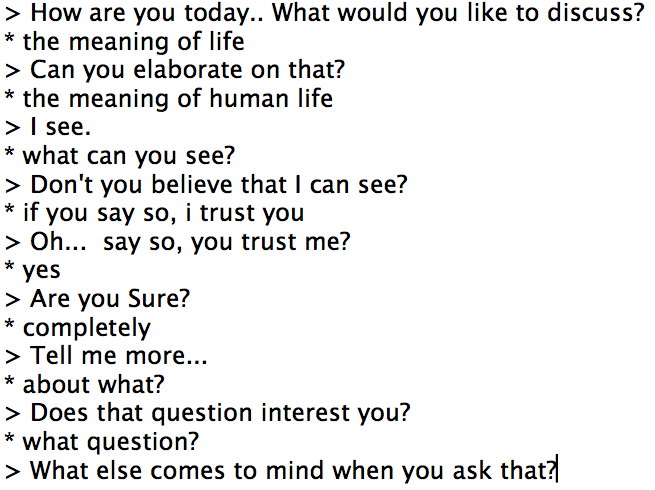
\includegraphics[width=0.5\textwidth]{eliza.png}
		\end{center}	
	Da la impresión de que Eliza te pide a ti que continúes la conversación (en vez de sacar un tema aleatorio como Alice), lo cual la da más apariencia de psicoanalista.
	
	\newpage
\begin{section}{Wolfram$\vert$Alpha}
	Según wikipedia:
	
	`Wolfram Alpha  es un buscador de respuestas desarrollado por la compañía Wolfram Research. Es un servicio en línea que responde a las preguntas directamente, mediante el procesamiento de la respuesta extraída de una base de datos estructurados, en lugar de proporcionar una lista de los documentos o páginas web que podrían contener la respuesta, tal y como lo hace Google.'
	
	Ciertamente trata de responder de manera directa cualquier pregunta, pero su potencial está ligado a las matemáticas y a la ciencia que a resolver cualquier pregunta curiosa ( de hecho su código está escrito en Mathematica). Eso sí, cada día es capaz de resolver más problemas y tratar más temas, pero las preguntas que puedes encontrar en Wikipedia o en Google directamente no tiene sentido irlas a buscar a una aplicación que es más lenta.  Aunque siempre que la forma en que introduzcas la pregunta sea correcta, si la temática ha sido añadida recibirás una respuesta satisfactoria.
	
	  Su potencia es increíble y crece día a día de manera impresionante. No podrás mantener una conversación sobre el clima de la semana, pero puede serte de mucha ayuda a la hora de tratar temas complejos como la química, las matemáticas, la física, la medicina, la informática o incluso el tiempo y la meterología. Eso sí, de dará la respuesta a la pregunta que le hagas, no te preguntará por el partido del Madrid de ayer.
	
	Por todas estas razones, y por el largo uso que llevamos dándole desde que entramos en la carrera, consideramos Wolfram Alpha como una de las herramientas  más inteligentes y útiles que existen, y un claro ejemplo de la importancia de la inteligencia artificial en el mundo actual.
	
	El gráfico de conocimiento de Google tiene gran utilidad cuando no tienes una buena conexión a internet porque cargar una búsqueda de Google no requiere la misma carga de datos que la página web donde tendrías que acceder a consultarlos. Además es más sencillo acceder a la información si te la muestran directamente y no tienes que buscarla dentro de la página donde está. 
	
	Creo que responde a una clara demanda de los usuarios y del mundo actual. Sin embargo aún le queda mucho por hacer a Google para conseguir algo que pueda compararse mínimamente con Wolfran Alpha.
	
	
\end{section}
	
	%\end{section}
	\end{itemize}
\end{section}
\begin{section}{Deep Blue y Walter}
	\begin{itemize}
		\item{\textbf{Deep Blue}}
		
		\begin{center}
		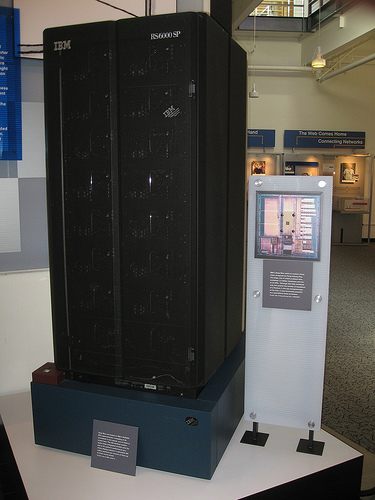
\includegraphics[width=0.3\textwidth]{deepBlue.png}
		\end{center}
		
		 Deep blue es una supercomputadora fabricada en los años 60 por IBM desarrollada para jugar al ajedrez, que en 1996 se enfrentó al campeón del mundo Gary Kaspárov. Consiguió vencerle una vez, pero al mejor de 6 Deep Blue fue vencido.
	
		Más tarde, una versión mejorada de Deep Blue, consiguió vencer a Kaspárov ajustadamente en un encuentro a 6 partidas. Aún así Kaspárov denunció irregularidades en estas partidas que nunca llegaron a ser explicadas por IBM. 

		La limitación de Deep Blue, realmente es la limitación que encuentran todas las máquinas que intentan jugar al ajedrez. El espacio de estados es enorme debido a la complejidad del juego, por lo que es imposible explorar todas las opciones hasta el final. Lo que hizo diferente a Deep Blue, además del bombo que le dio IBM que lo usó de escaparate para su empresa, fue que contaba con 30  microprocesadores y 480 procesadores especializados en el ajedrez. Sencillamente fue la máquina más potente que se dedicó al ajedrez en la época por lo que logró los mejores resultados. Era capaz de calcular 200 posiciones por segundo, que aunque daba una exploración limitada, dedicando suficiente tiempo era capaz de plantar cara al campeón del mundo.
	
	\newpage
	\item{\textbf{Watson}}
	
		\begin{center}
		\includegraphics[width=0.7\textwidth]{Watson.png}
		\end{center}
	
		Watson es un sistema informático de inteligencia artificial desarrollado por IBM diseñado para ser capaz de responder preguntas realizadas en lenguaje natural.
	
		Es famoso porque fue capaz de derrotar en el concurso televisivo \textit{Jeopardy!} al que más dinero había ganado en la historia del concurso y al que más programas seguidos había estado.
	
		Su principal limitación está en el tiempo que necesita para ser capaz de procesar una pregunta y responderla. Aun así fue capaz de vencer en el concurso gracias a la ejecución de miles de algoritmos distintos para la misma pregunta, lo que le permitía elegir la respuesta que más algoritmos encontrasen a la vez que cotejaba en su base de datos si la respuesta tenía sentido, y de esta forma aumentar la probabilidad de acierto para una respuesta dada. 
		
	\end{itemize}
\end{section}

\newpage
\begin{section}{Traducciones}

	\textit{Human beings solve most of their problems using fast, intuitive judgements rather than the conscious, step-by-step deduction that early AI research was able to model. AI has made some progress at imitating this kind of "sub-symbolic" problem solving: embodied agent approaches emphasize the importance of sensorimotor skills to higher reasoning; neural net research attempts to simulate the structures inside the brain that give rise to this skill; statistical approaches to AI mimic the probabilistic nature of the human ability to guess.}

	\vspace{0.5cm}

	Se traduce como:

	\vspace{0.5cm}

	\textit{Los seres humanos resuelven la mayor parte de sus problemas usando juicios intuitivos, rápidos en lugar de lo consciente, paso a paso deducción que las primeras investigaciones de AI fue capaz de modelar. Amnistía Internacional ha hecho algunos progresos en la imitación de este tipo de "sub-simbólico" la resolución de problemas: los agentes incorporados enfoques hacen hincapié en la importancia de sensoriomotoras habilidades de razonamiento superior; red neuronal investigación intenta simular las estructuras internas del cerebro que dan lugar a esta habilidad; enfoques estadísticos a AI imitan la naturaleza probabilística de la capacidad humana de adivinar.	}
	
	\vspace{0.5cm}

	El primer problema está en que al anteponer dos adjetivos (fast, intuitive) antes de un sustantivo, no ha detectado que ambos adjetivos van con dicho sustantivo, separando el primero tras una coma. Además traduce AI como Amnistía Internacional, que claramente no es lo que se pretende. Tampoco ha detectado que ``paso a paso'' debería ponerse a continuación de ``deducción''. Continúa habiendo fallos similares, luego en definitiva, cuando el texto a traducir es más complejo y no tiene frases sencillas, la aplicación estructura la traducción de manera incorrecta. 
	
	El principal problema es la interpretación: cuando un ser humano lee un texto y trata de comprenderlo, hay ocasiones en las que debe elegir qué significa un conjunto de palabras seguidas (como el ejemplo de ``fast, intuitive judgements''), pero tras un instante, es capaz de entender cuál de entre las opciones es la correcta, debido al contexto y a todos los textos anteriores que ha leído y comprendido. El computador, aunque tenga una gran memoria, es limitado, pues no es capaz de elegir por si mismo y simplemente computa en función de cómo esté programado, cuál es el significado correcto. Es un problema semántico. Y ya si intentamos traducir un texto literario:
	
\textit{Del salón en el ángulo oscuro, 
}	

\textit{de su dueña tal vez olvidada, 
}

\textit{silenciosa y cubierta de polvo 
}

\textit{veíase el arpa. 
}

\textit{¡Cuánta nota dormía en sus cuerdas 
}

\textit{como el pájaro duerme en las ramas, 
}

\textit{esperando la mano de nieve 
}

\textit{que sabe arrancarlas! 
}

\textit{¡Ay! pensé; ¡cuántas veces el genio 
}

\textit{así duerme en el fondo del alma, 
}

\textit{y una voz, como Lázaro, espera 
}

\textit{que le diga: «¡Levántate y anda!».
}

\vspace{0.5cm}

Google Translate lo traduce como: 

\vspace{0.5cm}

\textit{Of living in the dark corner, }

\textit{of its owner perhaps forgotten, }

\textit{Silent and dust cover} 

\textit{could be seen the harp. }

\textit{Note slept much on its strings }

\textit{as the bird sleeps in the branches, }

\textit{hand expecting snow} 

\textit{who knows pluck!} 


\textit{Ay! I thought;How many times the genius }

\textit{and sleeping in the depths of the soul, }

\textit{and a voice, like Lazarus, expected} 

\textit{you say, "Get up and walk!".}
	
\vspace{0.5cm}

Queda patente lo dicho.
	
\end{section}

	\newpage
\begin{section}{Aplicaciones informáticas inteligentes}

	Inteligente no sería la palabra correcta para describir estas aplicaciones, ya que realmente no tienen inteligencia, pero sí que son capaces de parecer muy inteligentes. La que mejor finge ser inteligente en una conversación normal es Alice, pues realmente es capaz de tener una conversación sobre los temas que más se tratan normalmente. Pero en lo que se refiere a inteligencia en su campo sin duda Wolfram Alpha el la mejor aplicación. Es capaz de resolver prácticamente cualquier ecuación, integral, derivada, interpolación o inferencia que se le proponga, siempre que sea resoluble. 
	
	Resumiendo, debido al poco conocimiento de inglés de Enrique Alice le parece la aplicación más inteligente. Sin embargo, para Iker que estudia actualmente en Bristol la más inteligente o que realiza mejor su función es Wolfram Alpha. Aunque si tiene que elegir un robot conversador será a SIRI, pues ninguno de los encontrados le convence, y su amor por apple resulta decisivo.
	
	El mundo espera un robot con el que poder hablar y que te haga la cama, pero aún queda  tiempo para conseguir comercializar algo parecido; aunque quizá menos del que pensamos.
		\begin{center}
		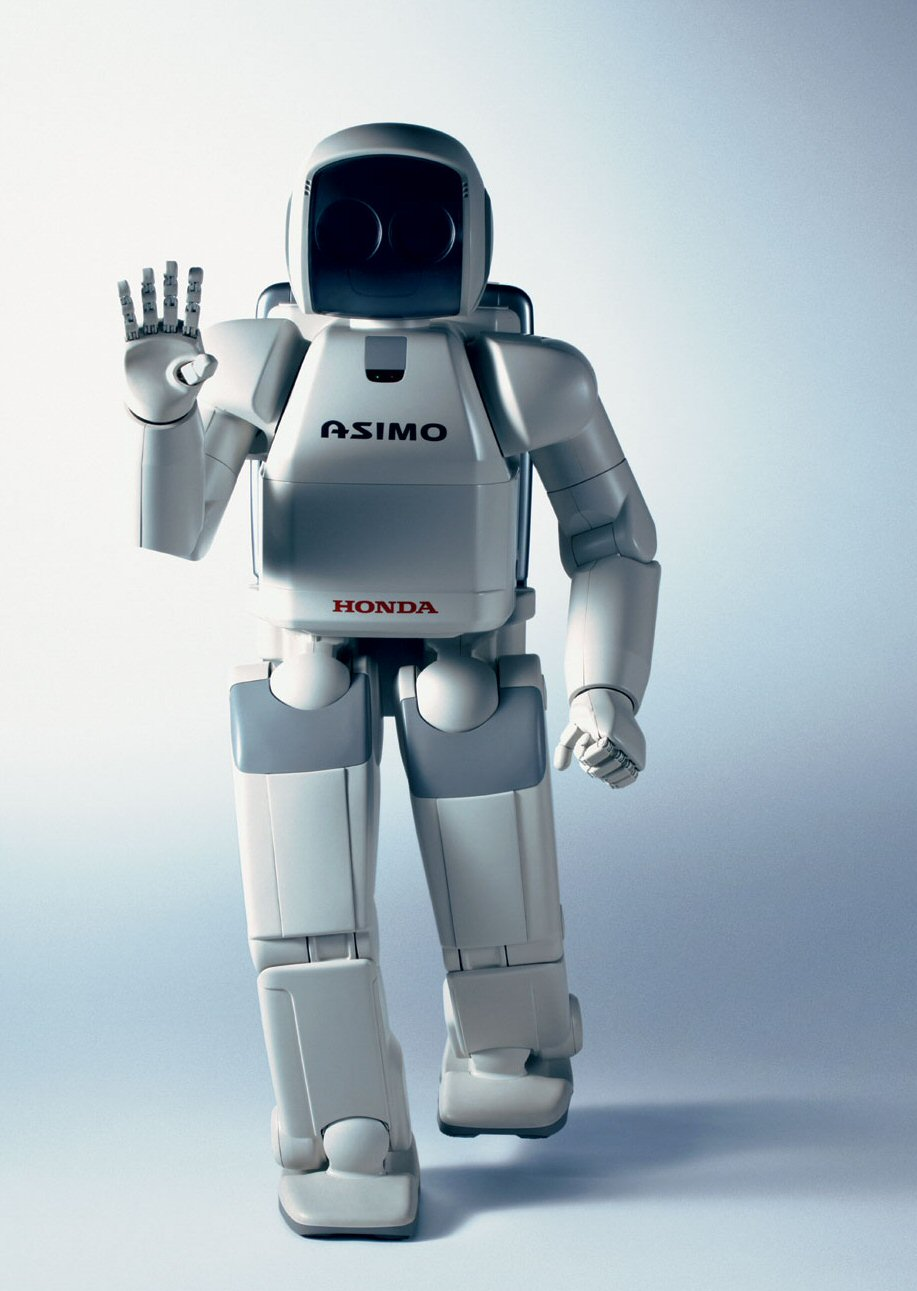
\includegraphics[width=0.4\textwidth]{asimoHonda2.png}
		\end{center}
	
\end{section}

\end{document}

